\documentclass[11pt]{article}

\usepackage[a4paper,margin=1in]{geometry}
\usepackage{amsmath,amssymb}
\usepackage{graphicx}
\usepackage{booktabs}
\usepackage[T1]{fontenc}
\usepackage[utf8]{inputenc}
\usepackage{textcomp}
\usepackage{natbib}
\usepackage{hyperref}
\usepackage{caption}
\hypersetup{colorlinks=true, linkcolor=blue, citecolor=blue, urlcolor=blue}

\title{MarxKapital: A Computational Framework for Marxian Value Theory\\
with Real Empirical Calibration}
\author{Nigel Randsley}
\date{July 2026}

\begin{document}
\maketitle

\begin{abstract}
We present MarxKapital, an open-source Julia package for the mathematical
modeling of Marxian value theory: capital accumulation, the tendency of the
rate of profit, the transformation of labor values into prices of
production, and the sectoral dynamics of expanded reproduction. Beyond the
classical two-department and generalized $N$-department reproduction
schemes, the package implements three complementary mechanisms for coupling
sectoral accumulation through the technical matrix~$A$ --- capital
mobility, an aggregate realization-pressure heuristic, and an exact
per-sector quantity-rationing scheme solved by fixed-point iteration ---
without recourse to differential-algebraic equation (DAE) solvers; the
rationing mechanism is validated numerically and demonstrated
qualitatively on a synthetic economy, but not yet against real
per-sector accumulation data, for which no suitable time series
currently exists. We
further present a live, reproducible empirical pipeline that calibrates the
model directly from official European statistical sources (Eurostat and
AMECO, via their SDMX REST APIs), replacing the synthetic or ad hoc
calibration common in the computational Marxian literature. Applying this
pipeline to Portugal, we document a sectoral profile for 2022 and an
aggregate profit-rate series for 1996--2022 in which the rate of
exploitation rises markedly while the organic composition of capital
falls, yielding a rising profit rate over the period --- a finding we
discuss critically rather than as a settled conclusion, given the
measurement conventions and simplifications involved.
\end{abstract}

\section{Introduction}

Empirical and computational work in the Marxian tradition faces a
recurring reproducibility problem: profit-rate and organic-composition
estimates in the literature are frequently produced by bespoke,
non-public spreadsheets or scripts, calibrated to data sources whose
vintage and exact construction are difficult to reproduce
\citep{shaikh2016capitalism,dumenil1993economics}. At the same time,
existing open computational implementations of Marxian reproduction
schemes tend to rely on synthetic or randomly generated sectoral data for
demonstration purposes, since assembling a real technical (input-output)
matrix, real sectoral value-added and employment series, and real capital
stock data from official sources is itself a substantial undertaking.

MarxKapital is an attempt to close both gaps at once. It is, first, a
methodological contribution: a Julia implementation of the classical
two-department reproduction scheme, its generalization to $N$ departments,
the labor-value and Sraffian production-price apparatus for the
transformation problem, and --- the paper's central technical
contribution --- three distinct mechanisms for coupling $N$-department
accumulation dynamics through the technical matrix, culminating in an
exact quantity-rationing scheme in the spirit of the disequilibrium-macro
literature \citep{barro1971general,benassy1975neokeynesian}, implemented
without the numerical machinery a literal differential-algebraic
formulation would require. This last mechanism is validated
numerically and demonstrated on a synthetic economy (Section~5.4); it
has not yet been tested against real per-sector accumulation data. It
is, second, an empirical contribution: a
live data pipeline that fetches real sectoral national accounts,
input-output tables, and macroeconomic series from Eurostat and the
European Commission's AMECO database via their official SDMX REST APIs,
and uses them to calibrate every quantity the model needs --- constant
and variable capital, the rate of exploitation, the organic composition,
the technical matrix itself, and (optionally) a perpetual-inventory
capital-stock series --- with no synthetic fallback unless explicitly
requested.

We use this pipeline to calibrate the model for Portugal and report two
sets of results: a detailed 19-sector profile for 2022, and an aggregate
time series of the rate of exploitation, organic composition, and profit
rate for 1996--2022. The latter shows a profit rate that rises over the
period, driven by a rate of exploitation that rises faster than the
organic composition falls. We present this as a genuine empirical finding
from real, unmodified official data, but discuss it critically: it runs
against the classical tendential-fall expectation, and we consider several
candidate explanations without asserting any of them as established.

The remainder of the paper is organized as follows. Section~2 situates the
model in the relevant theoretical literature. Section~3 presents the model
itself, including the coupled $N$-department dynamics and the
quantity-rationing mechanism. Section~4 describes the empirical
calibration pipeline and the Portuguese data. Section~5 reports results.
Section~6 discusses the findings and the model's limitations. Section~7
concludes.

\section{Related work}

The theoretical foundations implemented here are classical: the
reproduction schemes of \citet{marx1976capital1}, the tendency of the rate
of profit discussed in \citet{marx1981capital3}, and the transformation of
values into prices of production, for which we adopt the Sraffian
linear-production-price formulation of \citet{sraffa1960production}.
\citet{okishio1961technical} established the conditions under which
technical change and the choice of technique affect the profit rate, a
result the package's technical-matrix machinery is built to be consistent
with, though we do not implement an explicit choice-of-technique search.
On the empirical side, \citet{shaikh2016capitalism} and
\citet{dumenil1993economics} are the standard references for long-run
profit-rate estimation from national accounts; our approach differs mainly
in emphasizing a fully automated, re-runnable data pipeline over manual
series construction. Closer in spirit is the strand of empirical Marxian
work that estimates the profit rate and its components econometrically
from official national-accounts series over long time spans
\citep{basu2013reserve}, and the broader program of Marxian estimation
from harmonized international input-output databases such as the World
Input-Output Database; MarxKapital shares the latter's emphasis on a
real technical matrix rather than a value-only aggregate calibration,
but differs in coupling that matrix to explicit accumulation dynamics
rather than using it for static decomposition alone. The monetary-expression-of-labor-time
problem we flag in Section~5.3 is treated at length in
\citet{freeman1996marx}. The exact quantity-rationing mechanism introduced in
Section~3.3 draws on the disequilibrium-macroeconomics literature on
short-side rationing rules, in particular \citet{barro1971general} and
\citet{benassy1975neokeynesian}, applied here to a Leontief-technology
setting rather than the labor/goods markets those papers originally
analyze.

\section{The model}

\subsection{The classical two-department scheme}

The package's starting point is Marx's classical two-department scheme:
Department~I produces means of production, Department~II produces
consumption goods. Each department $d\in\{1,2\}$ is characterized by
constant capital $C_d$, variable capital $V_d$, and a rate of exploitation
$e_d$, giving surplus value $S_d = e_d V_d$, organic composition
$k_d = C_d/V_d$, and profit rate $r_d = e_d/(k_d+1)$. Accumulation follows
\begin{align}
  \dot C_d &= \sigma_{c,d} S_d - \delta_d C_d, &
  \dot V_d &= \sigma_{v,d} S_d,
\end{align}
where $\sigma_{c,d}+\sigma_{v,d}+\gamma_d=1$ splits surplus value between
reinvestment in constant capital, reinvestment in variable capital, and
capitalist consumption, and $\delta_d$ is a depreciation rate. Intersectoral
consistency (does Department~I's wage and unaccumulated-surplus income
suffice to buy Department~II's output, and vice versa) is checked
\emph{a posteriori} by a dedicated consistency function, not imposed
inside the differential system --- a design choice the $N$-department
generalization inherits and, in one respect, improves upon
(Section~3.3).

\subsection{Generalization to $N$ departments and the technical matrix}

For $N$ sectors, the model introduces a technical matrix $A\in\mathbb
R^{N\times N}_{\ge 0}$, with $A_{ij}$ the value of good $i$ required as
input per unit of output of sector $j$, constructed either synthetically
(with structural options for random, triangular, or block sparsity
patterns, always rescaled to spectral radius below unity) or --- our
empirical contribution --- from a real input-output table
(Section~4). Given $A$ and a labor-coefficient vector $l$, labor values
follow the Leontief inverse, $\lambda = (I-A)^{-1}l$, and Sraffian
production prices follow
\begin{equation}
  p = w(1+\bar r)\left[I-(1+\bar r)A^\top\right]^{-1} l,
\end{equation}
valid for any uniform profit rate $\bar r$ below the maximum feasible rate
$R_{\max} = 1/\lambda_{\max}(A^\top) - 1$, where $\lambda_{\max}$ denotes
the dominant eigenvalue. The baseline $N$-department accumulation system
treats sectors as independent, exactly mirroring the two-department
equations sector by sector; $A$ is available to the value/price apparatus
above but does not, in this baseline system, feed back into the
accumulation dynamics themselves.

\subsection{Coupling sectors through $A$: three mechanisms}

The baseline independence of sectors is a known limitation of purely
value-accounting reproduction models: physically, one sector's constant
capital is another sector's output, and the technical matrix should
constrain how much investment a sector can realize, not merely how its
value and price magnitudes are computed. MarxKapital implements three
progressively more demanding mechanisms to address this, all opt-in and
mutually composable except where noted, applied to a coupled system whose
accumulation equation for constant capital becomes
\begin{equation}
  \dot C_i = \kappa_i\,\sigma_{c,i} S_i - \delta_i C_i +
             \mu\,(r_i - \bar r)\, C_i,
  \label{eq:coupled}
\end{equation}
where $r_i$ is computed with constant capital valued at Sraffa production
prices (using the current aggregate profit rate, clamped below
$0.95\,R_{\max}$ to avoid the pricing singularity, with a labor-value
fallback if the price system is ill-conditioned) rather than raw book
value, so that $A$ enters the dynamics through valuation as well as
through the mechanisms below.

\paragraph{Capital mobility.} The term $\mu(r_i-\bar r)C_i$ reallocates
investment toward above-average-profit sectors, a direct computational
analogue of capital's tendency to flow toward higher returns.

\paragraph{Aggregate realization pressure.} Setting $\kappa_i \equiv
\min(\rho_{\text{real}},1)$ uniformly across sectors, with
$\rho_{\text{real}} = \sum_i \min(O_i,(AO)_i) / \sum_i (AO)_i$ and gross
output $O_i=C_i+V_i+S_i$, dampens planned reinvestment economy-wide
whenever aggregate intermediate demand implied by $A$ and current outputs
exceeds what those same outputs can supply. This is a coarse,
aggregate approximation --- it does not distinguish which sectors are
actually constrained --- but requires no iterative solution.

\paragraph{Exact per-sector quantity rationing.} The paper's central
technical contribution replaces the aggregate heuristic with a genuine
per-sector rationing scheme. Under Leontief technology, a sector's planned
reinvestment cannot substitute a shortage of one input with more of
another; realized investment is bounded by the scarcest required input,
and a sector's own shortfall reduces its effective demand for \emph{all}
its inputs, which in turn affects the rationing faced by its suppliers.
This makes the problem simultaneous. Writing $\rho_i\in(0,1]$ for the
rationing factor faced by \emph{suppliers} of good $i$ and $\kappa_j$ for
the realized fraction of planned reinvestment for \emph{buyer} $j$, the
fixed point is
\begin{align}
  \kappa_j &= \min_{i:\,A_{ij}>0} \rho_i, &
  D_i &= \sum_j A_{ij}\,\kappa_j\,\sigma_{c,j}S_j, &
  \rho_i &= \min\!\left(1, \frac{O_i}{D_i}\right).
\end{align}
We solve this by damped (under-relaxed) fixed-point iteration inside the
right-hand side of the ODE at every solver evaluation, in exactly the same
spirit as the Sraffa-price linear solve above, rather than exposing
$(\rho,\kappa)$ as differential-algebraic state to the solver. This choice
is deliberate: a literal DAE formulation (mass-matrix or index reduction)
or a general nonlinear-complementarity solver would add real numerical
risk and a new package dependency for no benefit over the fixed point,
which we verified converges reliably (a closed-form two-sector example
with a known solution $\rho_1=\sqrt{0.8}$, and no convergence failures
across more than twenty parameter combinations at $N=8$ and at $N=19$).
We emphasize that undamped iteration is \emph{not} reliable here: we
verified by hand that a small two-sector example oscillates indefinitely
between two states without under-relaxation, a concrete instance of the
well-known failure mode of naive Picard iteration on $\min$-based maps.

None of the three mechanisms imposes exact market clearing at every
instant for every sector as a hard constraint solved simultaneously with
the differential state --- that would require the DAE formulation we
deliberately avoid. A dedicated consistency-check function generalizes the
two-department \emph{a posteriori} check to $N$ sectors, reporting the
per-sector gap $O_i - (AO)_i$ and the aggregate realization ratio at a
given point in the trajectory, for diagnostic use outside the dynamics
themselves.

\section{Empirical calibration}

\subsection{Data sources}

MarxKapital fetches four families of real sectoral and macroeconomic data
\citep{eurostat_nama10a64,eurostat_naio10cp1620,ameco2026}, each via an
official SDMX REST API rather than a static file:

\begin{itemize}
  \item \textbf{Sectoral value added, compensation, and consumption of
    fixed capital} from Eurostat's national accounts by industry
    (\texttt{NAMA\_10\_A64}), at the 19-section NACE Rev.~2 level.
  \item \textbf{Sectoral employment and gross fixed capital formation}
    from the companion Eurostat datasets \texttt{NAMA\_10\_A64\_E} and
    \texttt{NAMA\_10\_A64\_P5}.
  \item \textbf{A real technical matrix} from Eurostat's symmetric
    input-output table at basic prices (\texttt{NAIO\_10\_CP1620}),
    product by product, aggregated to Leontief technical coefficients
    weighted by sectoral value added.
  \item \textbf{Aggregate macroeconomic series} (GDP, employment,
    compensation, capital stock, and eighteen further variables) from the
    European Commission's AMECO database.
\end{itemize}

All four sources were, until recently, distributed as static bulk files
with heuristic, undocumented formats; both institutions have since
migrated to
official SDMX REST APIs, which MarxKapital uses directly, with the legacy
static-file parsers retained only as a manual fallback.

\subsection{Constructing the technical matrix}

The symmetric input-output table records trade and transport margins as
part of national-accounting convention, which can produce negative entries
in the trade and transport product rows when the raw flows are aggregated
naively to a coarser sectoral grouping. We avoid this by building the
technical matrix at the full 19-sector resolution first --- where the
margin artifacts are confined to individual cells and can be clipped to
zero without discarding genuine flows from other sectors --- and only then
aggregating, when a coarser grouping is needed, using the standard
Leontief aggregation formula (value-added-weighted averaging of already
non-negative coefficients) rather than re-aggregating raw flows. The
resulting 19-sector matrix for Portugal is well behaved: non-negative
throughout, with spectral radius $\rho(A) \approx 0.13$ (Figure~2),
comfortably below unity.

\subsection{Depreciation and capital stock}

By default the model uses the net capital stock reported directly by
Eurostat for the requested year. As an option, it instead constructs a
perpetual-inventory series, $K_t = (1-\delta)K_{t-1} + I_t$, seeded from
the earliest year with both a reported stock and investment series, with
$\delta$ estimated per sector from the ratio of consumption of fixed
capital to stock in that base year rather than assumed. This uses a
single depreciation rate per sector, not differentiated by asset type; we
return to this simplification in Section~6.2.

\section{Results: Portugal}

\subsection{Sectoral profile, 2022}

Table~1 reports the calibrated rate of exploitation, organic composition,
and profit rate for all 19 sections, ranked by profit rate. The
value-added-weighted means are $e\approx0.89$, $k\approx24.8$, and
$r\approx10.0\%$; the mean organic composition is dominated by a single
outlier, real estate activities ($k\approx334$), which reflects the
well-known effect of imputed owner-occupied rents inflating capital
intensity in this sector's national-accounts treatment rather than a
genuine production characteristic, and should be discounted accordingly
when interpreting the sectoral mean. Excluding real estate, sectoral
profit rates range from financial and insurance activities at the top
($r\approx36\%$) to public administration and utilities near the bottom
($r$ below 2\%), a dispersion consistent with the classical expectation
that market prices, not labor values, equalize profit rates across
sectors of differing organic composition --- which Section~5.3 examines
directly.

\begin{table}[htbp]
\centering
\caption{Sectoral calibration, Portugal, 2022 (real Eurostat data).}
\begin{tabular}{llrrrr}
\toprule
Code & Sector & VAB (M\texteuro) & $e$ & $k$ & $r$ (\%) \\
\midrule
K & Financial and insurance activities & 23.2 & 1.51 & 3.17 & 36.1 \\
S & Other service activities & 5.0 & 0.62 & 1.97 & 20.83 \\
I & Accommodation and food service & 33.8 & 0.86 & 3.51 & 19.07 \\
G & Wholesale and retail trade & 54.8 & 0.53 & 2.05 & 17.37 \\
A & Agriculture, forestry and fishing & 16.3 & 1.39 & 8.3 & 14.98 \\
N & Administrative and support & 16.0 & 0.33 & 1.28 & 14.37 \\
F & Construction & 19.8 & 0.33 & 1.61 & 12.65 \\
M & Professional, scientific and technical & 21.2 & 0.34 & 1.79 & 12.23 \\
C & Manufacturing & 88.0 & 0.53 & 3.91 & 10.75 \\
B & Mining and quarrying & 3.2 & 0.65 & 9.44 & 6.19 \\
J & Information and communication & 25.1 & 0.22 & 2.84 & 5.71 \\
P & Education & 21.6 & 0.1 & 1.08 & 4.8 \\
Q & Human health and social work & 34.4 & 0.1 & 1.93 & 3.41 \\
H & Transportation and storage & 43.3 & 0.23 & 6.33 & 3.13 \\
L & Real estate activities & 382.3 & 8.52 & 333.82 & 2.55 \\
E & Water supply, sewerage, waste & 15.6 & 0.34 & 13.78 & 2.3 \\
R & Arts, entertainment and recreation & 7.9 & 0.12 & 4.15 & 2.29 \\
O & Public administration & 88.5 & 0.1 & 7.45 & 1.18 \\
D & Electricity, gas, steam & 33.4 & 0.1 & 62.91 & 0.16 \\
\bottomrule
\end{tabular}

\end{table}

\subsection{Aggregate profit-rate trend, 1996--2022}

Figure~1 shows the aggregate rate of exploitation, organic composition,
and profit rate for Portugal over 1996--2022, calibrated entirely from
real AMECO series. The rate of exploitation rises from $0.21$ to $0.61$;
the organic composition falls from $8.99$ to $5.40$; the profit rate rises
correspondingly from $2.1\%$ to $9.5\%$. We discuss this finding in
Section~6.1.

\begin{figure}[htbp]
\centering
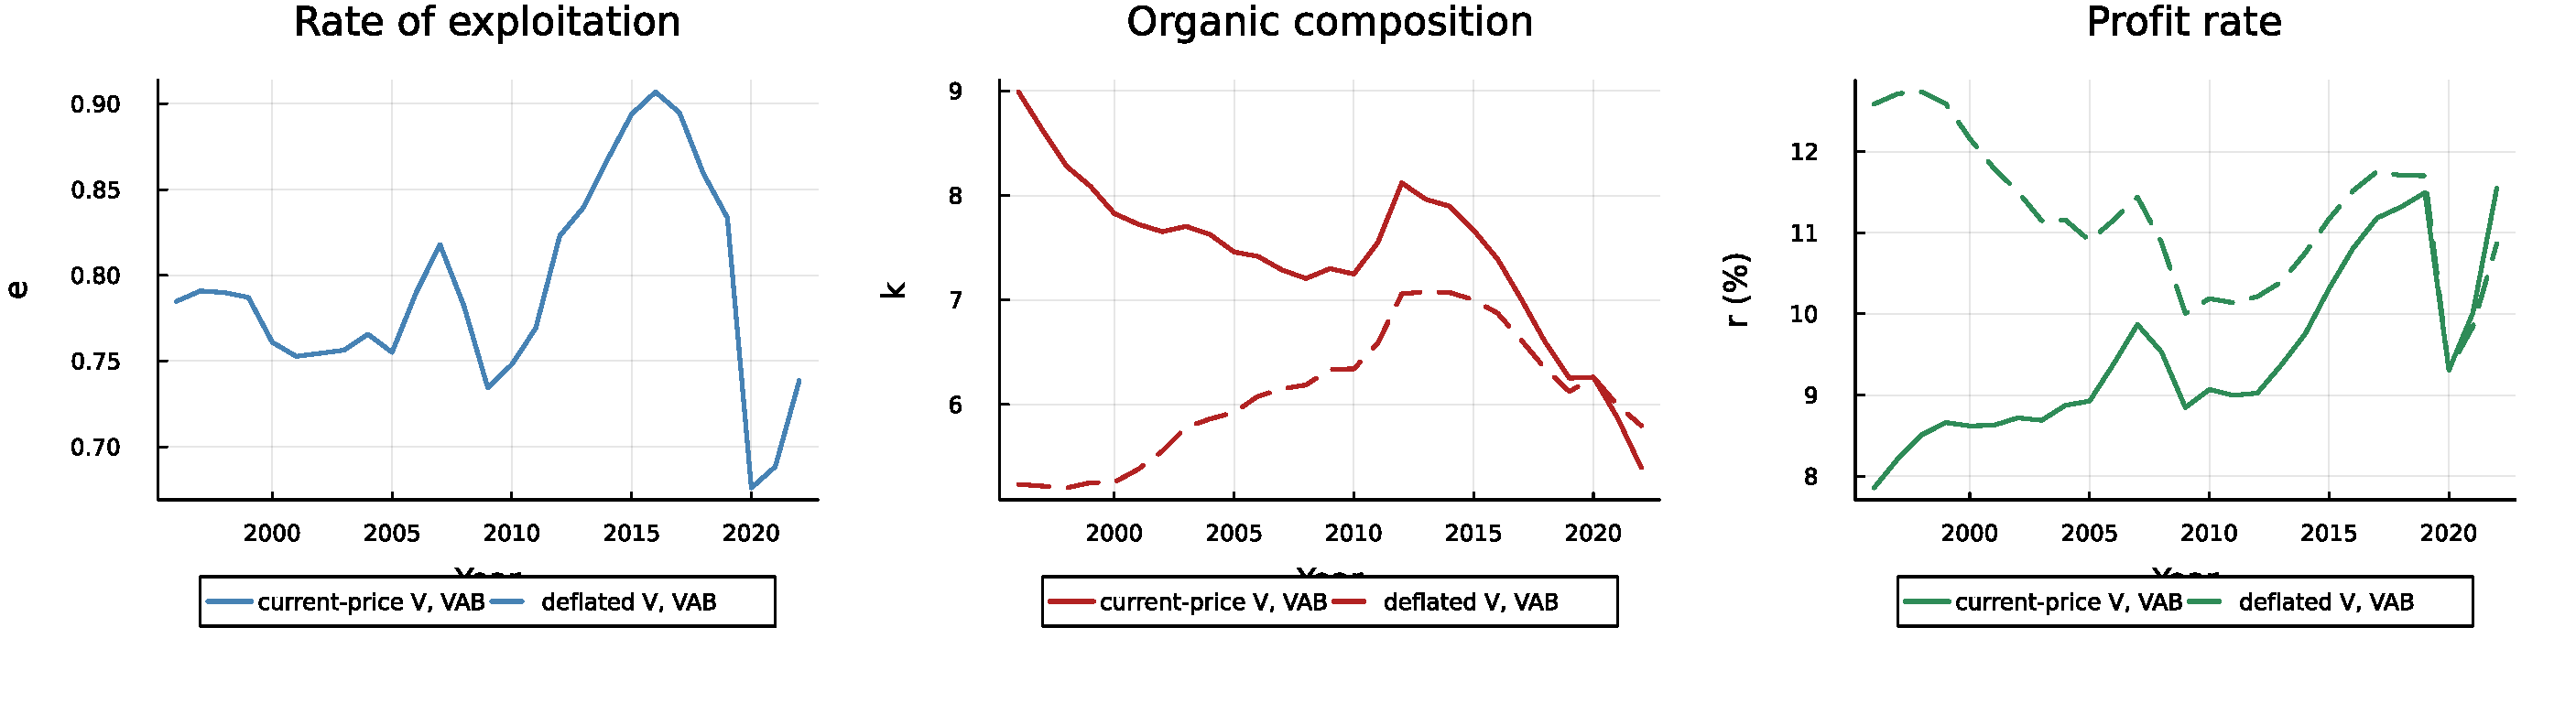
\includegraphics[width=\textwidth]{figures/fig1_time_series.pdf}
\caption{Rate of exploitation, organic composition, and profit rate,
Portugal, 1996--2022 (real AMECO data).}
\end{figure}

\begin{figure}[htbp]
\centering
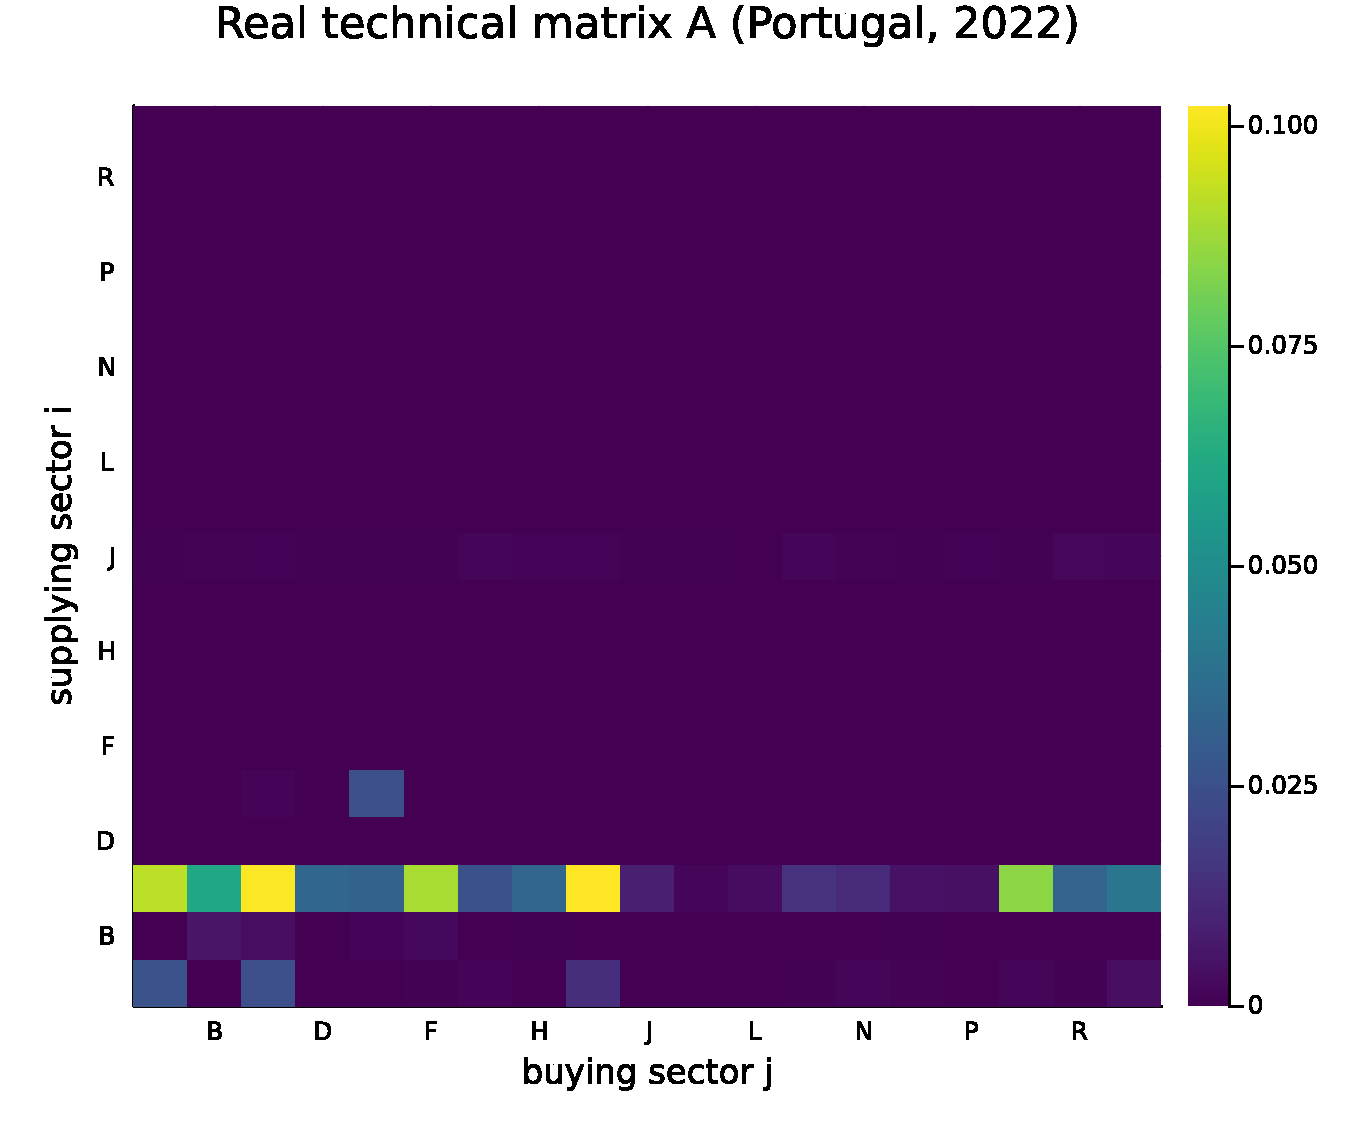
\includegraphics[width=0.7\textwidth]{figures/fig2_matrix_A.pdf}
\caption{Real technical matrix $A$, Portugal, 2022 (19 NACE sections).}
\end{figure}

\subsection{The transformation problem on the real economy}

Figure~3 compares labor values with Sraffian production prices computed
on the real calibrated matrix, for three illustrative uniform profit rates
($\bar r = 0$, $0.3R_{\max}$, $0.6R_{\max}$, with $R_{\max}\approx691\%$
for this economy). As $\bar r$ rises, sectors with above-average organic
composition see their production price rise relative to their labor
value, and vice versa, the qualitative signature the transformation
problem predicts, now shown on a real rather than a randomly generated
technical structure. The comparison is qualitative only: labor values
are expressed in labor-time units and production prices in the
wage-numeraire monetary units of Equation~2, and we do not fix an
explicit monetary expression of labor time (MELT) to convert between
them. Figure~3 therefore reports each series normalized to sum to one
and compares relative deviations, which is sufficient to display the
sign and ordering of the transformation effect but does not license a
literal price-value comparison in a common unit --- a well-known
difficulty in empirical Marxian value theory
\citep{freeman1996marx,basu2013reserve}.

\begin{figure}[htbp]
\centering
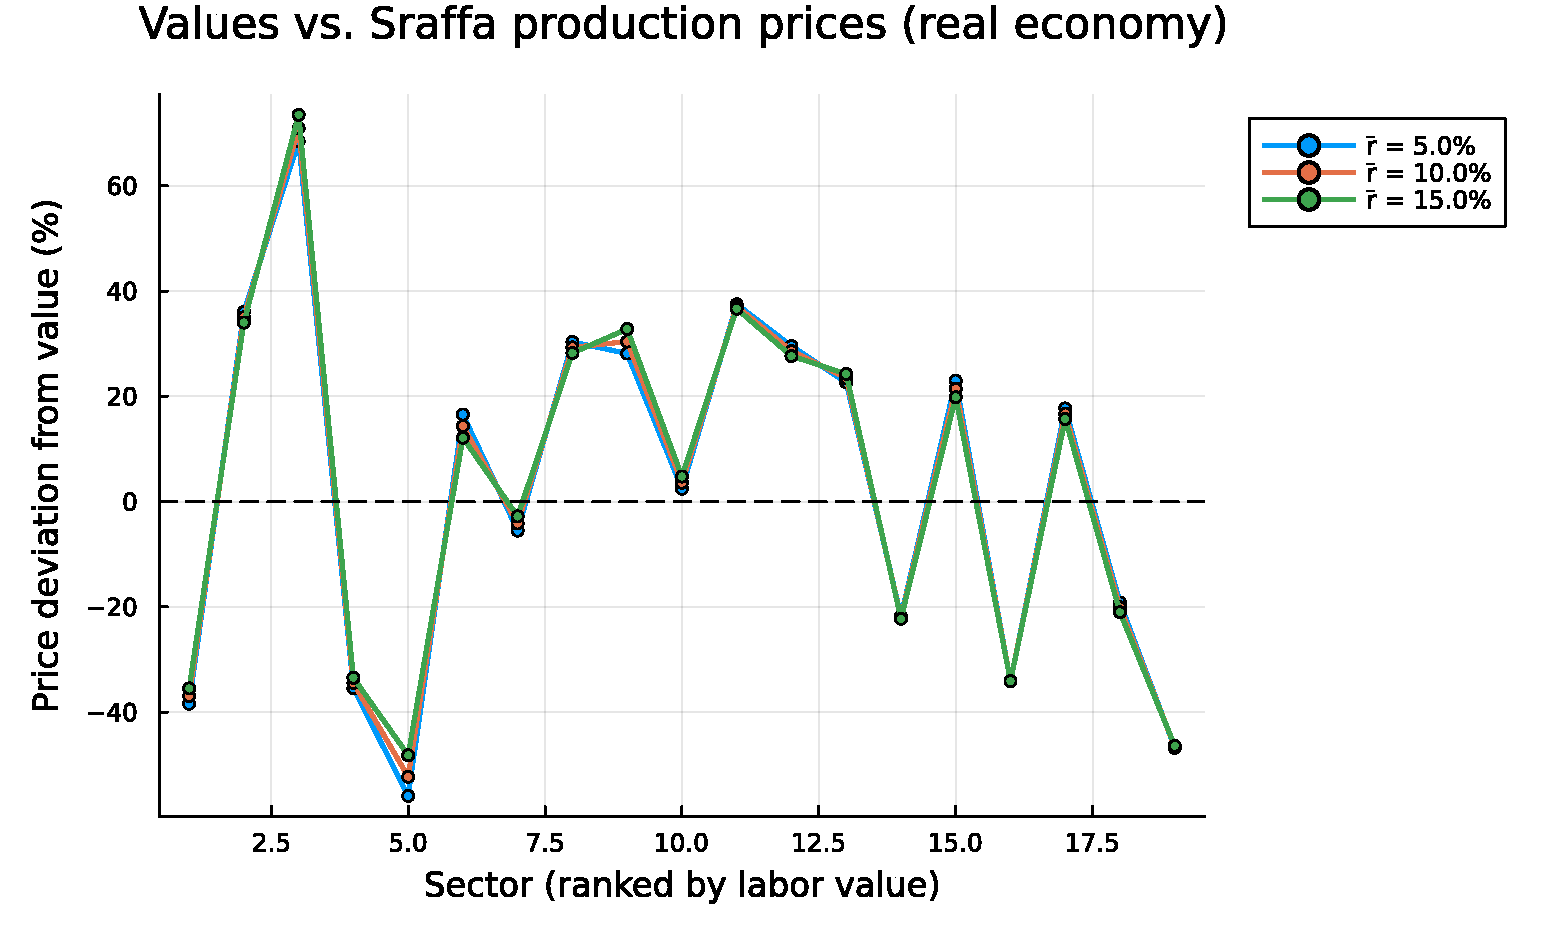
\includegraphics[width=0.75\textwidth]{figures/fig3_transformation.pdf}
\caption{Labor values vs.\ Sraffian production prices, real technical
matrix, Portugal 2022, at three illustrative profit rates.}
\end{figure}

\subsection{Illustrative comparison of coupling mechanisms}

Because no real per-sector accumulation time series exists to calibrate
the dynamic coupling mechanisms of Section~3.3 empirically, Figure~4
illustrates their qualitative behavior on a synthetic six-sector economy
under a common random technical matrix and seed. Capital mobility alone
reduces cross-sector profit-rate dispersion over time, as expected.
Adding the aggregate realization-pressure term leaves the qualitative
picture largely unchanged in this run. Adding exact quantity rationing
instead \emph{increases} final dispersion relative to mobility alone in
this particular random economy: rationing can prevent the mobility term
from fully equalizing rates when a high-profit sector's own suppliers
cannot support the investment mobility would otherwise direct there. We
report this honestly as an example of the mechanism's behavior rather than
evidence that rationing systematically increases or decreases dispersion
in general --- the result is specific to this synthetic economy's random
technical structure, and a systematic characterization across many random
economies is left for future work.

\begin{figure}[htbp]
\centering
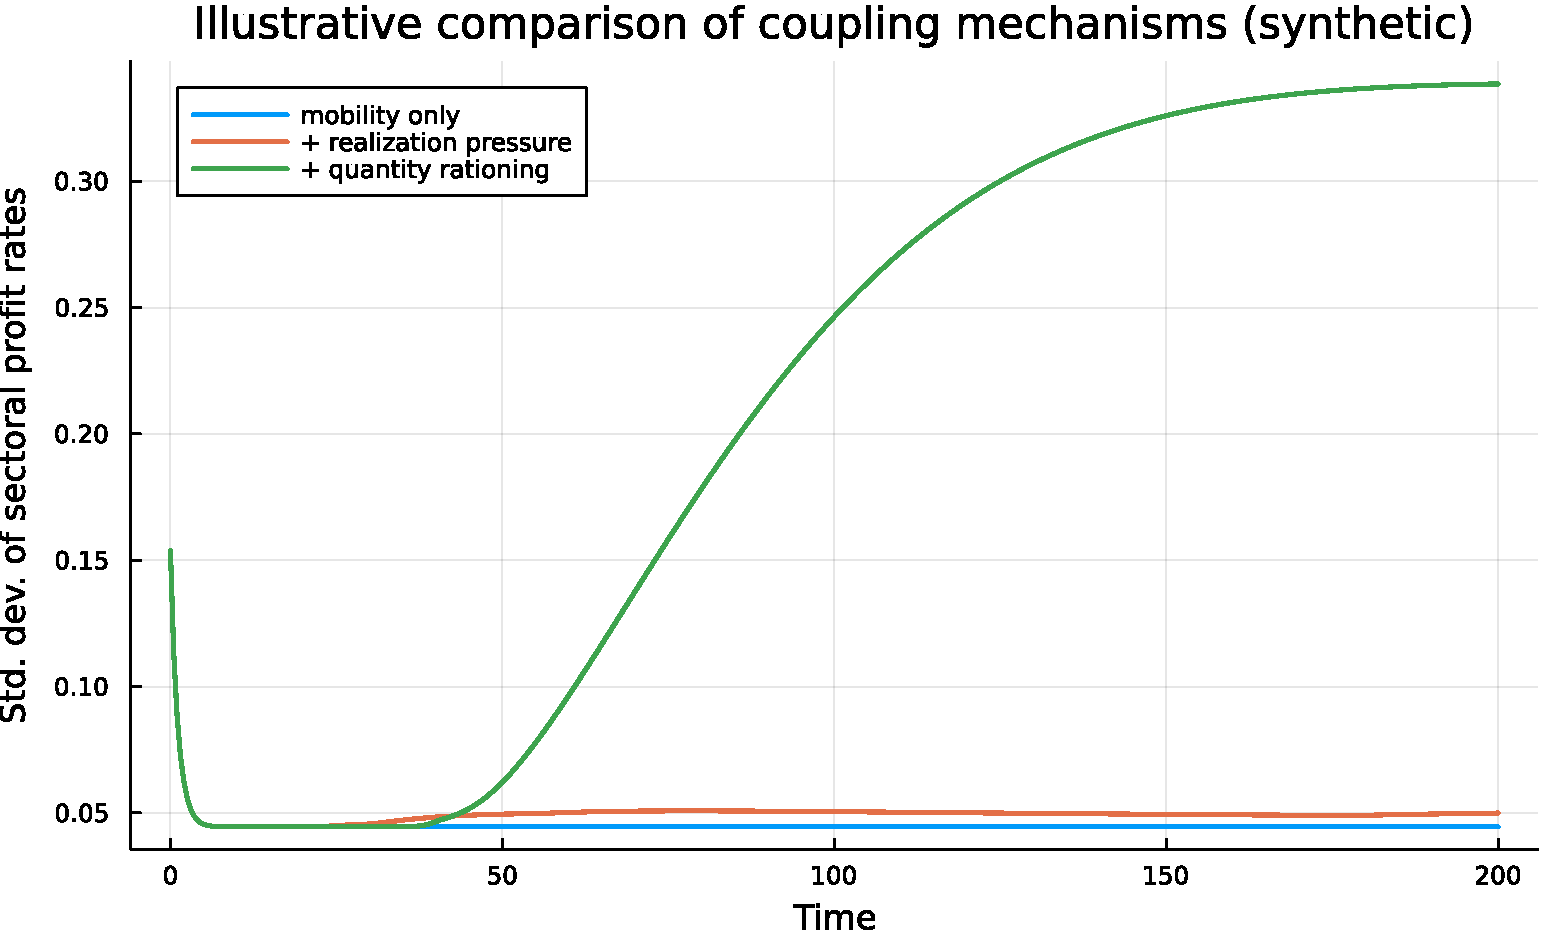
\includegraphics[width=0.75\textwidth]{figures/fig4_coupling_comparison.pdf}
\caption{Cross-sector profit-rate dispersion over time under three
coupling mechanisms (illustrative synthetic economy, not calibrated to
real data).}
\end{figure}

\section{Discussion}

\subsection{Interpreting the rising profit rate}

The rising profit rate found for Portugal over 1996--2022 runs counter to
the classical tendential-fall expectation, in which a rising organic
composition is expected to depress the profit rate faster than a rising
rate of exploitation can offset it. Here the opposite pattern holds: the
organic composition \emph{falls} over the period, and the rate of
exploitation rises enough on its own to more than compensate. We consider
this a genuine empirical finding from unmodified official data, not an
artifact of the calibration pipeline, but we do not consider it a settled
interpretation of underlying economic processes. Several non-exclusive
candidate explanations are worth further investigation: intensified
exploitation associated with wage moderation and labor-market
liberalization over the period, including during the 2011--2014 assistance
programme; capital-saving technical change, plausible given the economy's
structural shift toward less capital-intensive services; compositional
effects from Portugal's deepening integration into EU-wide production
networks; and a measurement effect specific to how the organic
composition is constructed here. AMECO's capital-stock series is
expressed in current prices, and the organic composition it implies is
therefore a \emph{value} composition, not a \emph{technical} one: decades
of relative price decline in capital goods --- computing equipment,
machinery, software --- can push a current-price capital/labor ratio
down even with no change, or an increase, in the underlying physical
capital/labor ratio, a distinction long stressed in the empirical
Marxian literature \citep{shaikh2016capitalism,basu2013reserve}. We
cannot rule this out with the current pipeline, since it does not yet
support a constant-price capital stock; repeating the calibration with a
volume-deflated series, rather than the current-price AMECO default, is
the most direct way to test whether the falling organic composition
survives a switch from value to technical composition, and is a natural
next step before treating the finding as more than suggestive.
Distinguishing between these is beyond the
scope of this paper and would require disaggregating the aggregate series
by sector and comparing against the 2022 cross-section of
Table~1 --- itself complicated by the single-year nature of the sectoral
calibration versus the time-series nature of the aggregate result.

\subsection{Limitations}

We report limitations transparently, following the same practice as the
package's own documentation.

\emph{Default behavior remains synthetic.} Both calibration paths default
to synthetic data or fixed sectoral weights; every real-data result in
this paper required explicit opt-in flags. This is a deliberate design
choice to keep the package's automated test suite fully offline, not a
limitation of the real-data pipeline itself, but it means synthetic
results should never be mistaken for empirical ones when using the
package's defaults.

\emph{Single-rate depreciation.} The perpetual-inventory capital-stock
option (Section~4.3) uses one depreciation rate per sector, not
differentiated by asset type. Eurostat publishes investment by asset type
for the relevant dataflow, but not the corresponding asset-specific
depreciation profiles, which would be needed for a fully differentiated
perpetual-inventory calculation.

\emph{No microfoundation for final demand.} The quantity-rationing
mechanism of Section~3.3 constrains reinvestment demand through the
technical matrix but does not model how aggregate consumption demand is
allocated across sectors, since no data source in the current pipeline
provides sector-of-origin consumption baskets. The mechanism should
therefore be read as constraining the investment-goods side of
reproduction specifically, not final demand in general.

\emph{Coarser sectoral aggregations inherit a data-quality caveat.} When
the technical matrix is aggregated from 19 to 3 macro-sectors, the
tertiary (services) row is conservative because it inherits reduced
intermediate-flow estimates for the trade and transport sub-sectors,
whose margin-accounting convention we clip at the finer resolution before
aggregating (Section~4.2); the coarser matrix is non-negative and usable,
but likely understates services' true role as an input supplier to other
sectors.

\emph{No systematic robustness or sensitivity analysis.} The results
above are reported for a single set of parameter choices: net capital
stock rather than perpetual-inventory, current-price rather than
volume-deflated valuation, and, for the coupling mechanisms of
Section~3.3, a single value of the mobility coefficient $\mu$ and a
single random seed. We likewise report the 1996--2022 trend for
Portugal alone; whether the pattern is Portugal-specific or shared
across peripheral EU economies (Spain being the obvious comparator,
using the identical AMECO pipeline) is untested. The fixed-point
convergence claim in Section~3.3 is empirical, based on a finite set of
parameter combinations, not a proof; a formal contraction argument
under stated conditions on $A$, $\sigma$, and $\delta$ would strengthen
it considerably. We regard all of these as the most direct next steps
before treating either the empirical trend or the rationing mechanism's
qualitative behavior as more than suggestive.

\section{Conclusion}

MarxKapital demonstrates that a real, live, officially sourced data
pipeline for Marxian value-theoretic calibration is practical using
current European statistical infrastructure, and that exact per-sector
market-clearing dynamics can be added to a reproduction-schema model
without the numerical overhead of a formal differential-algebraic
formulation. Applied to Portugal, the pipeline surfaces a genuine and, we
think, under-examined empirical pattern --- a rising profit rate driven by
rising exploitation outweighing falling organic composition --- that
merits further sectoral and comparative investigation beyond the scope of
this paper.

\section*{Availability}

MarxKapital is released under the MIT license. The complete source code,
including the empirical pipeline described here, is available at
\url{https://github.com/randsley/MarxKapital}. Every figure and table in
this paper is produced, without manual editing, by
\texttt{paper/gerar\_resultados.jl}, which performs live queries against
the Eurostat and AMECO SDMX APIs; re-running it reproduces this paper's
results from the same official data sources.

\bibliographystyle{plainnat}
\bibliography{references}

\end{document}
